
%\input{$HOME/YData/lectures/ydata_lecture_styles}
\input{../../lectures/ydata_lecture_styles}



%%%TITLE SLIDE (defined in style file)
\tslide{10}{Groups}


%%%SLIDE
\frame{
\begin{center}
\huge \tt Announcements
\end{center}
}


%%%SLIDE
\frame{
\begin{center}
\huge \tt Example:  Predictions
\end{center}
}

%\begin{center}
%\alert{(DEMO)}
%\end{center}

%%%SLIDE
\frame{
{Sir Francis Galton}

\begin{minipage}{0.6\textwidth}
\begin{itemize}
\item 1822 - 1911 (knighted in 1909)
\item A pioneer in making predictions
\item  Particular (and troublesome)
interest in heredity
\item Charles Darwin's half-cousin
\end{itemize}
\begin{center}
\alert{(DEMO)}
\end{center}
\end{minipage}
%
\begin{minipage}{0.38\textwidth} \centering
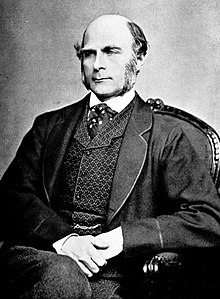
\includegraphics[width = \textwidth]{francis_galton.png}
\end{minipage}
}

%%%SLIDE
\frame{
\begin{center}
\huge \tt  Apply with Multiple Columns
\end{center}
}


%%%SLIDE
\frame{
{Apply}
The {\tt  \color{Blue} apply} method creates an array by calling a function on every element in input column(s)
\begin{customlist}{2em}{0em}
\item First argument: \quad \quad Function to apply
\item Other arguments: \quad The input column(s)
\end{customlist}
\bigskip

{\color{Blue} \tt
table\_name.apply(one\_arg\_function, `column\_label') \\
%
table\_name.apply(two\_arg\_function, \\
\hspace{3cm} `column\_label\_for\_first\_arg',\\
\hspace{3cm}  `column\_label\_for\_second\_arg')
}
\bigskip

{\tt  \color{Blue} apply} called with only a function applies it to each row
\vfill
\begin{center}
\alert{(DEMO)}
\end{center}
}



%%%SLIDE
\frame{
\begin{center}
\huge \tt   Grouping by One Attribute
\end{center}
}


%%%SLIDE
\frame{
{Grouping by One Column}

The {\tt \color{Blue} group} method aggregates all rows with the same value for a column into a single row in the resulting table.
\bigskip
\begin{customlist}{0em}{0em}
\item First argument: Which column to group by
\bigskip
\item Second argument: (Optional) How to combine values
\begin{itemize}
\item {\tt \color{Blue} len} -- number of grouped values (default) 
\item {\tt \color{Blue} list} -- list of all grouped values
\item {\tt \color{Blue} sum} -- total of all grouped values
\end{itemize}
\end{customlist}
\vfill
\begin{center}
\alert{(DEMO)}
\end{center}
}


%%%SLIDE
\frame{
\begin{center}
\huge \tt    Cross-Classification
\end{center}
}


%%%SLIDE
\frame{
{Grouping By Multiple Columns}

The {\tt \color{Blue} group} method can also aggregate all rows that share the combination of values in multiple columns

\begin{customlist}{2em}{0em}
\item First argument: \quad \quad A list of which columns to group by
\item Other arguments: \quad (Optional) How to combine values
\end{customlist}
\vfill
\begin{center}
\alert{(DEMO)}
\end{center}
}


%%%SLIDE
\frame{
\begin{center}
\huge \tt   Pivot Tables
\end{center}
}




%%%SLIDE
\frame{
{Pivot}

\begin{customlist}{0em}{0em}
\item Cross-classifies according to two categorical variables
\bigskip
\item Produces a grid of counts or aggregated values
\bigskip
\item Two required arguments:
\begin{itemize}
\item First: variable that forms column labels of grid
\item Second: variable that forms row labels of grid
\end{itemize}
%
\bigskip
\item Two optional arguments (include both or neither)
\begin{itemize}
\item {\tt {\color{Blue} values} = `column\_label\_to\_aggregate'}
\item {\tt c{\color{Blue} ollect} = function\_with\_which\_to\_aggregate}
\end{itemize}
\end{customlist}
\vfill
\begin{center}
\alert{(DEMO)}
\end{center}
}


%%%SLIDE
\frame{
{Challenge Question}
Which NBA teams spent the most on their ``starters'' in 2015-2016? \\
Assume the ``starter'' for a team \& position is the player with the highest salary on that team in that position.

\begin{center}
\begin{tabular}{|c|c|c|c|}
\hline
{\bf PLAYER} & {\bf POSITION} & {\bf TEAM} & {\bf SALARY} \\
\hline
Paul Millsap & PF & Atlanta Hawks & 18.6717 \\
\hline
Al Horford & C & Atlanta Hawks & 12 \\
\hline
Tiago Splitter & C & Atlanta Hawks & 9.75625 \\
\hline
\end{tabular}
\end{center}
\vfill
\begin{center}
\alert{(DEMO)}
\end{center}
}


%%%SLIDE
\frame{
{Take-Home Question}
Generate a table of the names of the starters for each team

\begin{center}
\includegraphics[width = \textwidth]{nba_table.png}
\end{center}
}


%\frame{ 
%{References} \footnotesize
%\bibliographystyle{$HOME/YData/bibliography/asa}
%\bibliography{$HOME/YData/bibliography/ydata_bibliography}
%}
\end{document}
